\documentclass[handout,utf8]{article}
\usepackage{default}
\usepackage{tipa}
\usepackage{lingsty}
\usepackage{ipashortcuts}
\usepackage[authoryear]{natbib}  
\usepackage{graphicx}
%opening
\title{Catch me if you can: convergence towards a moving target}
\author{Sebastian Nordhoff}


\begin{document}

\maketitle
 
\begin{abstract}
 
\end{abstract}

\section{Introduction}

\section{Convergence}
Convergence is generally seen as two languages becoming more like another. \citet{Mattheier1996}, however, holds that in many cases, it is better to speak of `advergence', as there is usually one language which changes a lot in the direction of the other, while the other changes hardly at all. 

A clear case of advergence would be Pennsylvania Dutch, which becomes more like English, whereas the surrounding varieties of English are hardly influenced by Pennsylvania Dutch. A clear case of convergence would be Kupwar \citep{Gumperz}, where all three languages (Urdu, Kannada, Marathi) underwent change in the direction of the others. 

In this paper, I want to discuss language change processes in Sri Lanka and show that, depending on the subvarieties,  there are multiple advergence processes going on in conflicting directions. This network of changes makes it difficult to exactly locate the origin of a change. For instance, Sinhala, at a broad level, converges towards Tamil. Certain (Muslim) Tamil dialects, however, converge towards Sinhala. Sri Lanka Malay, finally, converges towards these Muslim Tamil dialects. If we find  a feature X in Sri Lanka Malay, how can we say whether it comes directly from Tamil, whether it comes from Tamil via Sinhala, or whether it comes from Sinhala via Muslim Tamil? 

This paper is structured as follows: I will first give an overview of the Sri Lankan linguistic ecology, sketching the sociolinguistic, geographic and demographic setup of the relevant languages and giving some historical background. I will then discuss received wisdom about the contact situation. After taking a look at the dialectology of the respective languages, I will reassess the contact situation, showing that the language change processes are more complex than assumed. 

\section{The Sri Lankan linguistic ecology}
The first language spoken in Sri Lanka that we know of is the \textbf{Vedda} language \ref{}. Various proposals have been made as to its origins, but as a matter of fact, language attrition has proceeded to a point where little of any substance can be said about the affiliation of this language. Vedda as spoken today can be considered a variety of Sinhala with some lexical and morphological peculiarities \citep{abc}. Due to the lack of material, Vedda will not be considered further in this paper. 

Sinhala (Indo-Aryan) and Tamil (Dravidian) both arrived on the island about three millennia ago, although the respective order of arrival is a matter of heated debate. Sinhala has been shown to share some features with Western Indo-Aryan languages like Gujarati and others with Eastern Indo-Aryan languages like Bengali \citep{Geiger}. This suggests two waves of immigration, but again the chronological order is unsure. 

\begin{figure}
\begin{center}
 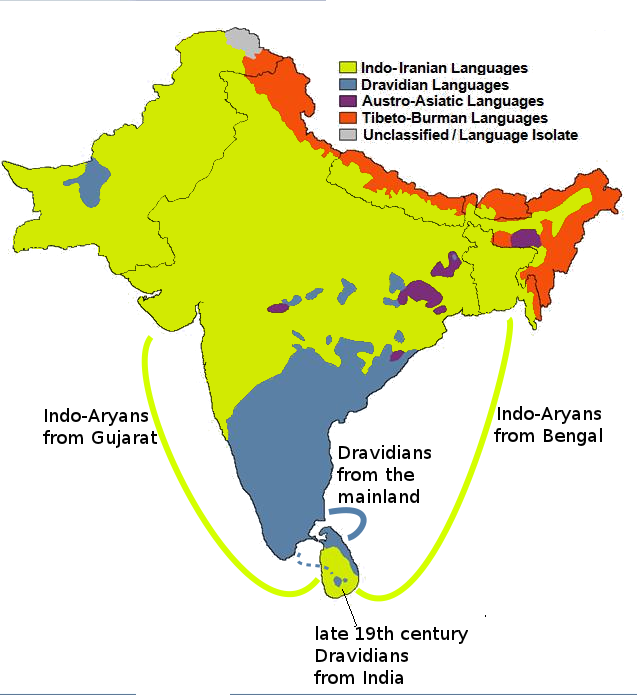
\includegraphics[height=.5\textheight]{insl.png}\end{center}
 \caption{Migrations from India to Sri Lankan}
\end{figure}

\textbf{Sinhala} is separated from its Northern cousins by the Dravidian languages of South India and is isolated within the family (disregarding Dhivehi (Maldivian), which is an offshoot of Sinhala). Due to prolonged contact with Dravidian languages, Sinhala became much more Dravidianized than any other Indo-Aryan language. In fact, the Indo-Aryan nature of Sinhala is so well concealed that in the 19th century, \citep{Rask1811} classified Sinhala as a Dravidian language. 

\citet{Gair} adds Sinhala to the South-South Asian Sprachbund, which comprises Southern India, Sri Lanka, and the Maldives. Features which set off Sinhala from the Northern Indo-Aryan languages are absence of aspirates, long \=e and \=o, conjunctive participles without a same-subject requirement, evidentials, quotatives, and a very thorough left-branching structure. These features are shared with Tamil.

Sinhala is today the majority language of Sri Lanka with about 74\% of the population speaking it as first language. Sinhala speakers are Buddhists or Christians. They mainly live in the West, Center, and South of the island, but can be found elsewhere as well. After the end of the Sri Lankan Civil War, there are ideas of settling Sinhala speakers in the Northern regions as well, which are predominantly Tamil.

\textbf{Sri Lankan Tamil} prides itself as a very old and pure form of this language. Tamil is spoken by the Sri Lankan Tamils (Hindu or Christian) mainly in the North, the Moors (Muslim) in the West and in cities, and the Indian Tamils (Hindu or Christian) in the central tea estates. These varieties differ considerably. Altogether, about 25\% of the Sri Lankan population speak one variety of Tamil as their mother tongue. 
Sri Lankan Tamil uses the same script and orthography as Indian Tamil, but spoken Sri Lankan Tamil is not intelligible to speakers from India. The differences are so important that speakers from India frequently think that their interlocutor does not speak a variety of Tamil at all, but rather Malayalam. It should also be noted that Tamil is a diglossic languages, and that written Tamil differs considerably from any variety of spoken Tamil. 

Jaffna Tamil is the most prestigious variety of Tamil on the island. Its main features are archaic phonology and morphology, a threefold deictic contrast, and a more differentiated negation system than Indian Tamil. The other varieties of Tamil on the island tend to be eclipsed by Jaffna Tamil in scholarly domains. We will return to this below. 

\textbf{Sri Lanka Portuguese} arrived on the island during the Portuguese period (1503-1656) as a Creole. Due to intermarriage with the local population, the language became thoroughly Lankanized and is now the only Creole with a European lexifier to have SOV word order or postpositions. The Dutch (1656-1798) continued to use Sri Lanka Portuguese as a lingua franca, a practice which continued into the early days of British rule (1798-1948). As a lingua franca, Sri Lanka Portuguese was also acquired by populations which otherwise had no connections to the colonial administration. Today, Sri Lanka Portuguese is spoken on the East Coast (Tamil-dominated) by about 4000 Portuguese Burghers, and by a very small number of Sri Lankan Kaffirs (descendants of slaves) on the West Coast. \citet{Smith} shows that the Burghers' Sri Lanka Portuguese is thoroughly influenced by Tamil. \citet{Hettiaratchi} refers to a recording of a centenary speaker of Sri Lanka Portuguese in the Sinhala dominated region, whose speech shows 
more influence from Sinhala. 


\textbf{Sri Lanka Malay} is the language of the descendants of immigrants brought during the Dutch and British period. It was mainly spoken in the centers of colonial administration, i.e. cities and towns in the center and in the South. Towards the end of the 19th century, Sri Lanka Malays were also employed as overseers on the emerging tea estates in the central Hill Country. Sri Lanka Malay has been argued to show influence from Muslim Tamil and/or from Sinhala. 

Sri Lanka Malay is relatively homogeneous. There is a small pocket of Sri Lanka Malay speakers on the South coast (Kirinda and Hambantota), which has some dialectal differences, but overall mutual intelligibility is good. 

% \textbf{Sri Lankan English} is the last language to develop on the island. It has mostly been treated within sociolinguistics. Studies of Sri Lankan English have focused on the Colombo variety, influenced by Sinhala. Work by \citet{Kumaraswamy} shows, that Sri Lankan English as spoken by Tamils differs from the variety portrayed in most linguistic work.
% Besides a peculiar phonology and lexical influences from the local languages, the syntax of Sri Lankan English has also been heavily influenced by the local languages.


\section{Who goes where, 1st iteration}
The standard view about language contact in Sri Lanka is that all languages that get there converge towards Tamil. This assumption is based on the observation that Sri Lankan Tamil is an archaic variety \citep{Zvelebil1959II}, which suggests that it has not changed a lot. Given that Sri Lanka is a sprachbund \citep{Bakker2012}, potentially within a larger South-South-Asian Sprachbund \citep{Gair2012}, the logical conclusion is that all other members have converged to the archaic language, Tamil in this case. This is received wisdom for Sinhala \citep{Geiger, Gair, Elizarenkova1972}, Sri Lanka Portuguese \citep{Smith, Jayasuriya} and Sri Lanka Malay \citep{Hussainmiya, Smith, Bakker}. Exclusive Tamil influence in Sri Lanka Malay has been challenged recently \citep{Ansaldo, Nordhoff}.\footnote{The oldest language of Sri Lanka, Vedda, is moribund and heavily sinhalized. Besides noting attrition, little more can be said about the language contact phenomena at work.}


\section{A closer look at the contact situations}
While at first sight, it appears that Tamil provides the typological sink all languages of the island move towards to, closer look at the actual varieties in question casts doubt on this scenario. I will now delve deeper into the internal diversity of the languages of the island and show, that at a closer look, the language change processes a far more complex than presented beforehand. 

\subsection{Sinhala}
Tamil influence on Sinhala syntax is clear and widely accepted. The phonological features of long mid vowels and lack of aspiration also distinguish Sinhala from Northern Indo-Aryan languages, and make it appear closer to Tamil. This led \citet{Elizarenkova1972} to argue for an extensive phonological influence from Tamil on Sinhala. In a very detailed study, however, \citet{Gair1976}, drawing on material by \citet{Karunatillake}, shows that all the mentioned changes towards Tamil were accompanied by changes \em away \em from Tamil in the very same periods. For instance, retroflex sonorant were lost in Sinhala despite Tamil having them. Furthermore, vowel length was first lost, despite Tamil showing this feature, only to be reintroduced later and so on.

\subsection{Tamil}
The internal diversity of Tamil is very high. The first division to be made is between written Tamil and spoken Tamil. In the context of this paper, written Tamil is not relevant. Spoken Tamil  can be divided into Indian Tamil (with further subdivisions) and Sri Lankan Tamil. Sri Lankan Tamil is not intelligible to Indians. The reverse is not true, due to the exposure to Tamil media and television. 

Within Sri Lanka, the most prestigious variety is Jaffna Tamil, spoken by Hindus and Christians. Next to Jaffna Tamil, the varieties of Trincomalee and Batticaloa also deserve mention. These varieties can clearly be distinguished. Tamil as spoken by Muslims differs from the variety used by the Hindus and Christians. Muslim Tamil itself is divided into a North-Eastern variety, close to Batticaloa Tamil, and a South-Western variety, which is heavily Sinhalized. 

Another Sinhalized variety is Negombo fishermen's Tamil \citep{Bonta}, which, like South-Western Muslim Tamil has lost verbal agreement. 

Things are further complicated by Indian migrant workers in the central tea estates, who arrived in the late 19th century. They spoke Indian dialects of Tamil (and other Dravidian languages), and their speech today is still closer to Indian Tamil than to Sri Lankan Tamil. Among these dialects, processes of dialect levelling probably took place \citet{abc}, but this is in need of further research. 

As far as language change is concerned, the varieties of Jaffna, Trincomalee and Batticaloa are generally seen as archaic, with little or nor change towards Sinhala having taken place. Muslim Tamil shows Arabic influence in the lexicon, and South-Western Muslim Tamil and Negombo fishermen's Tamil show syntactic incluence from Sinhala. 

Estate Tamil varieties are underresearched.


\subsection{Sri Lanka Malay}
Sri Lanka Malay shows quite a great deal of internal variation, but this variation does not pattern geographically. Serious differences in phonology, morphology or syntax can be found within the same town. The only clear regional difference observed up to know is a much more contracted speech in Hambantota and Kirinda on the South coast as compared to the other varieties. 



\subsection{Sri Lanka Portuguese}
Sri Lanka Portuguese dialectology has not been studied extensively. The major division is between the Eastern variety of the Portuguese Burghers and the Western variety of the Ceylon Kaffirs. The latter variety is likely to have undergone more influence from Sinhala, but it is moribund, so the extent of this influence is difficult to ascertain. Within the Burgher variety, the varieties of Trincomalee and Batticaloa are very close, but some morphological differences set them apart, e.g. the imperative marker. In all varieties, there is lexical influence from Tamil, and to a lesser extent, from Sinhala. 

\section{Who goes where, 2nd iteration}
Wrapping up what has been said in the previous section, we can state the following:

\begin{enumerate}
 \item Vedda changed towards Sinhala
 \item Sri Lanka Malay changes towards South-Western Muslim Tamil 
 \item South-Western Muslim Tamil changes towards Sinhala
 \item Negombo Tamil changes towards Sinhala. 
 \item Sinhala changes towards Tamil 
 \item Sri Lanka Portuguese changes towards Tamil in the East and West, and probably changed towards Sinhala in the West.
% \item Sri Lankan English changes towards Sinhala
\end{enumerate}

If we take point 2, we can say that Sri Lanka Malay changes towards (a variety of) Tamil, which is received wisdom. If we add point 3, it suddenly appears that Sri Lanka Malay changes towards Sinhala, via South-Western Muslim Tamil. But if we finally add point 5, it appears that the ultimate target is Tamil again. It is thus very difficult to catch the exact language change target of Sri Lanka Malay, as the target is ever-moving, and none of the relevant varieties are static enough to allow firm conclusions. 





\section{Conclusion}
        Convergence is an idealization
        Languages change, so the target changes as well
        The Sri Lankan situation is especially complex
        The multiple convergence processes are very hard to disentangle and often make it impossible to trace a borrowed structure to exactly one language
    Addendum
        SLE

\end{document}

\section{Convergence: the easy way}

  

\frame{
\frametitle{Sinhala}
% \begin{columns}
% \column{5cm}
\begin{itemize}
 \item  Sinhala is quite deviant from the Nothern Indian languages
\begin{itemize}
 \item long e, o 
 \item no aspirated stops k$^h$ t$^h$ p$^h$ etc \citep{Elizarenkova1972}
 \item no postposed relative clauses \citep[204]{Gair1998someremarks}
 \item focus construction \citep{Gair1985calque}
 \item ``[S]ubordinate verbal structures as a whole are of a strikingly Tamil and Dravidian character ...  the cumulative effect is nothing short of overwhelming'' \citep{Gair1998someremarks}
\item quotative \citep{Gair1998someremarks}
%  \item no copula
\end{itemize}
 \item in fact, the membership of Sinhala in Indo-Aryan was contested in the 19th century \citep{Tennent1859,Geiger1938}
\end{itemize}
% \columns{5cm}
% \end{columns}
}

\frame{
\frametitle{Sinhala}
% \begin{columns}
% \column{5cm}
\begin{itemize}
  \item \citet{Elizarenkova1972} explains the phonological facts  by Tamil influence
  \item Tamil has long mid vowels and lacks aspiration
  \item $\to$ Sinhala has converged towards Tamil
  \item will return to this topic below
\end{itemize}
% \columns{5cm}
% \end{columns}
}

\frame{
\frametitle{Sri Lanka Portuguese}
% \begin{columns}
% \column{5cm}
\begin{center}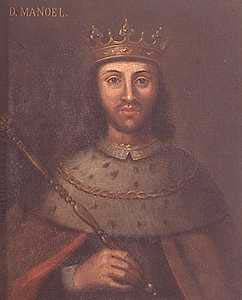
\includegraphics[height=.8\textheight]{Manuel.jpg} \end{center}
% Manuel.jpg: 242x300 pixel, 100dpi, 6.15x7.62 cm, bb=

% \columns{5cm}
% \end{columns}
}

\frame{
\frametitle{Sri Lanka Portuguese}
% \begin{columns}
% \column{5cm}
\begin{itemize}
 \item spoken at the East Coast in Batticaloa \citep{Smith1979}
 \item un-Romance
  \begin{itemize}
   \item features features
  \end{itemize}

 \item in contact with Tamil
 \item Tamil wives learnt Portuguese
 \item substrate influence
 \item convergence towards Tamil
\end{itemize}
% \columns{5cm}
% \end{columns}
}

\frame{
\frametitle{Sri Lanka Malay}
% \begin{columns}
% \column{5cm}
\begin{itemize}
 \item SLM has a very similar structure to SLP
 \item ergo the same origin
%  \item Tamil wives married Malay soldiers
 \item substrate influence
 \item convergence towards Tamil
\end{itemize}
% \columns{5cm}
% \end{columns}
}

\frame{
\frametitle{Conclusion of the easy way:}
% \begin{columns}
% \column{5cm}
\begin{itemize}
 \item {\LARGE All languages in Sri Lanka converge towards Sri Lankan Tamil}
\end{itemize}
% \columns{5cm}
% \end{columns}
}

\frame{
\frametitle{}
% \begin{columns}
% \column{5cm}
\begin{itemize}
 \item Break
\end{itemize}
% \columns{5cm}
% \end{columns}
}

\section{Areal linguistics: the painful way}

\frame{
\frametitle{Areal linguistics, the painful way}
% \begin{columns}
% \column{5cm}
\begin{itemize}
 \item
\end{itemize}
% \columns{5cm}
% \end{columns}
}

\frame{
\frametitle{Areal linguistics, the painful way}
% \begin{columns}
% \column{5cm}
\begin{itemize}
 \item what Tamil are we talking about?
  \begin{itemize}
   \item ``Standard (Indian) Tamil''? \citep{Schiffman1999}
   \item ``In Sri Lanka, the notion of accepting or not accepting  the ``unifying'' ability of S[tandard] S[poken] T[amil] is another matter, since SST is understood but not accepted as an intercaste mode of communication among Sri Lankan Tamils. This matter will not be resolved until the civil war in that island has ended.'
   \item Sri Lanka Tamil
     \begin{itemize}
   \item ``Standard Sri Lanka Tamil''?
   \item \citet[170f]{Gairdonotuse}: ``There is, in fact, more dialect variation within  Tamil in Sri Lanka than there is within the majority (Indo-Aryan) language Sinhala.''
   \item ``It happens  quite frequently that, when speaking about  Ceylon(ese) Tamil, what authors have really in mind is (one dialect of ) \em Jaffna \em Tamil. This should of course be avoided''\citep[137]{Zvelebil1966} 
     \end{itemize}
  \end{itemize}
% \item ``We can hardly speak of any dialectal difference of the Sinhalese language in the Island itself''\citep[168]{Geiger1938}
\end{itemize}
% \columns{5cm}
% \end{columns}
}

\frame{
\frametitle{The ethnography of Tamil in Sri Lanka}
% \begin{columns}
% \column{5cm}
\begin{itemize}
 \item conservative
  \begin{itemize}
   \item Jaffna: prestigious, Christian/Hindu \citep{Zvelebil1959II,Kuiper1962,Pillai1962,Zvelebil1966,Jaffna,Gairdonotuse}
   \item Trincomalee: Hindu  \citep{Zvelebil1959I,Zvelebil1966,Trincomalee}
   \item Batticaloa:  Hindu (literary-like)/Muslim \citep{Zvelebil1966,Batticaloa}
  \end{itemize}
 \item new
   \begin{itemize}
    \item mixed common Ceylonese \citep{Zvelebil1959II,Zvelebil1966} 
   \end{itemize}
 \item deviant
    \begin{itemize}
     \item Negombo: no person inflection \citep{Bonta2004,Bonta2008}
    \end{itemize}
\end{itemize}
% \columns{5cm}
% \end{columns}
}

\frame{
\frametitle{The ethnography of Tamil in Sri Lanka (cont.)}
% \begin{columns}
% \column{5cm}
\begin{itemize}
 \item Muslim Tamil \citep{Nuhman2007}
\begin{itemize}
 \item North Eastern Muslim Tamil: conservative
 \item South Western Muslim Tamil: convergence towards Sinhala
 \begin{itemize}
  \item loss of inflection; loss of retroflex \nz{} and \lz \citep{Nuhman2007}
 \end{itemize}
 \item immigrant Tamil \citep{conference}
 \begin{itemize}
  \item estate Tamil: Indian features (onglides, syncopation) \citep{Gairdonotuse}
 \end{itemize}
\end{itemize}'
\end{itemize}
% \columns{5cm}
% \end{columns}
}
% 
% \frame{
% \frametitle{The relation between Sinhala and Tamil}
% % \begin{columns}
% % \column{5cm}
% \begin{itemize}
%  \item \citet{Gair1985dravidianization} replies to Elizarenkova
%  \item It is true that a number of changes have made Sinhala look more like Tamil
%  \item however, things are more difficult than they look
%  \item many concomitant changes one would expect have not occured
%  \begin{itemize}
%   \item devoicing blablabbla
%  \end{itemize}
%  \item Sinhala language history shows acquistion of Dravidian and Undravidian phonological features in rapid succession, which is difficult to reconcile with unidirectional convergence
% \end{itemize}
% % \columns{5cm}
% % \end{columns}
% }

\frame{
\frametitle{Sri Lanka Portuguese}
% \begin{columns}
% \column{5cm}
\begin{itemize}
 \item SL Portuguese stands as described as converged towards conservative varieties of Tamil (Batticaloa)
\end{itemize}
% \columns{5cm}
% \end{columns}
}

\frame{
\frametitle{Sri Lanka Malay}
    \begin{itemize}
 \item SLM has become more South Asian
 \item Sinhala and Tamil share many structures \citep{Smith2003}
 \item What looks like Tamil influence could turn out to be Tamil influence
 \item What looks like Sinhala influence could turn out to be Tamil influence
    \begin{itemize}
    \item If there is Sinhala influence on SLM, it could be called ``Dravidian through the back door'' because of earlier Tamilization of Sinhala
    \end{itemize}
\end{itemize}
}

\frame{
\frametitle{Which variety of Tamil is a contact language for SLM?}
\begin{columns}
\column{6cm}
\begin{itemize}
 \item The Malays had no contact to the more conservative varieties of Tamil because of geography
 \item Hindu or Christian prestige do not count for Malays (or Moors for that matter)
 \item contact varieties: generalized SL Tamil, Negombo Tamil, South West Muslim Tamil
 \item those are precisely the varieties that are Sinhalized
 \item the latter varieties' influence can be called ``Sinhala influence through the back door''
\end{itemize}
\column{4cm}
\begin{center}
 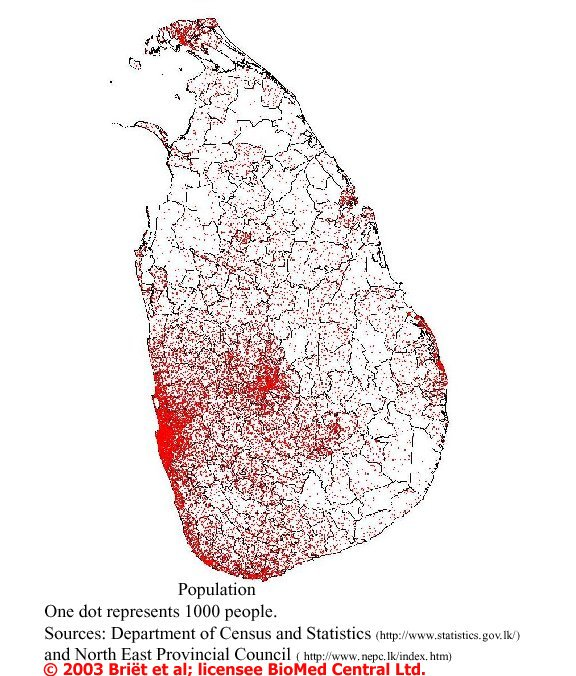
\includegraphics[height=.8\textheight]{./srilanka-pop-map.jpg} 
\end{center}

\end{columns}
}

\frame{
\frametitle{Cascading influences on Sri Lanka Malay: catch me if you can}
% \begin{columns}
% \column{5cm}
\begin{itemize}
 \item Malay converges towards SW Muslim Tamil\\
 ~~~~$\rightharpoonup$ SW Muslim Tamil converges towards Sinhala\\
 ~~~~~~~~$\rightharpoonup$ Sinhala converges towards general Dravidian structure 
\end{itemize}
% \columns{5cm}
% \end{columns}
}

\frame{
\frametitle{Cascading influences on Sri Lanka Malay: catch me if you can}
% \begin{columns}
% \column{5cm}
\begin{itemize} 
 \item Traditional definition of convergence: the involved varieties become more like each other
 \item Sri Lanka: at bird's eye view
 \begin{itemize}
  \item Sinhala goes Tamil
  \item Tamil remains inert
 \end{itemize}
 \item at closer view
  \begin{itemize}
   \item at closer view, Sinhala goes Dravidian
   \item Tamil varieties diverge and become \em less \em like each other
  \end{itemize} 
 \item Malay is in the middle of the confusion
\end{itemize}
% \columns{5cm}
% \end{columns}
}



% \frame{
% \frametitle{Conclusion} 
% \multiinclude[+>]{lggraph-}
% }%

% \frame{
% \frametitle{Conclusion}
% 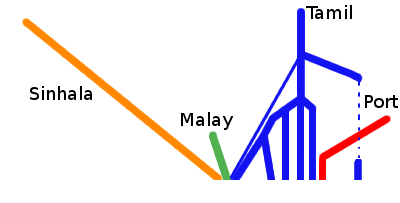
\includegraphics[width=\textwidth]{lggraph.mng}
% }

% 
% \frame{
% \frametitle{Conclusion}
% \includegraphics<1>[width=\textwidth]{lggraph-0.png}
% \includegraphics<2>[width=\textwidth]{lggraph-1.png}
% \includegraphics<3>[width=\textwidth]{lggraph-2.png}
% \includegraphics<4>[width=\textwidth]{lggraph-3.png}
% \includegraphics<5>[width=\textwidth]{lggraph-4.png}
% \includegraphics<6>[width=\textwidth]{lggraph-5.png}
% \includegraphics<7>[width=\textwidth]{lggraph-6.png}
% \includegraphics<8>[width=\textwidth]{lggraph-7.png}
% \includegraphics<9>[width=\textwidth]{lggraph-8.png}
% \includegraphics<10>[width=\textwidth]{lggraph-9.png}
% \includegraphics<11>[width=\textwidth]{lggraph-10.png}
% \includegraphics<12>[width=\textwidth]{lggraph-11.png}
% \includegraphics<13>[width=\textwidth]{lggraph-12.png}
% \includegraphics<14>[width=\textwidth]{lggraph-13.png}
% \includegraphics<15>[width=\textwidth]{lggraph-14.png}
% \includegraphics<16>[width=\textwidth]{lggraph-15.png}
% \includegraphics<17>[width=\textwidth]{lggraph-16.png}
% \includegraphics<18>[width=\textwidth]{lggraph-17.png}
% \includegraphics<19>[width=\textwidth]{lggraph-18.png}
% }

\frame{
\frametitle{Illustration} 
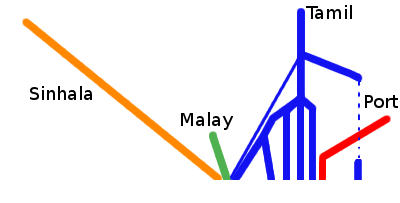
\includegraphics[width=\textwidth]{lggraph-18.png}
}

\frame{
\frametitle{The moving target}
% \begin{columns}
% \column{5cm}
\begin{itemize}
 \item linear convergence is not an option for Malay because of the moving target
 \item Sri Lanka Malay targets Tamil varieties which are on their way towards Sinhala which is on its way to yet other Tamil varieties
 \item The simple solution ``Everybody goes Tamil, and so does Malay'' is conceptually simplistic and underestimates the internal complexity of Sri Lankan Tamil ethnography
 \item Tamil and Sinhala are already difficult to tell apart in their standard variety
 \item In this complex dialect situation, it is close to impossible to tease apart what is Sinhala and what is Tamil in the local languages, including Tamil and Sinhala
 \item For the time being, it seems advisable to take into account both Tamil and Sinhala features in analyzing SLM data, allowing for Tamil influence through Sinhala and Sinhala influence through Tamil
\end{itemize}
% \columns{5cm}
% \end{columns}
}

% \bibliographystyle{natuva}
% \bibliography{ansaldo,asw,creole,india,phon,malay,sinhala,tamil,nordhoff,lankahist}

\frame{
\frametitle{Conclusion}
% \begin{columns}
% \column{5cm}
\begin{itemize}
 \item 
\end{itemize}
% \columns{5cm}
% \end{columns}
}

\tiny

Anonymous (s.a.).
\newblock \emph{tamiZH akaraatiyil (Tamil Lexicon) uLLa yaZHppaNac coRkaLin
  aayli}.
\newblock Ph.D. thesis, ilangkaip palk laikkaZHa kattu vittiyalangkaara
  vaLaakattil moZHiyavil.
\newblock KiRappuk kaLaiooaTTattiR ku?ya oaTangkaLuL onNuka iv aaylukkaTTirai
  camarppikkappaTTiLLatu cuTTilakkam ilankaip palk laik kaZHikam
  vittiyakangkaara vaLaakam.


Anonymous (1978).
\newblock \emph{tirukooNamaLai kiLaimoZhi}.
\newblock Ph.D. thesis.
\newblock MoZHiyiyalla ci?ppukkalaippaTTattiRku toortiterutta paaTangka?L o??ka
  ikkaTTirai cayarppikkappaTTinnata celvi civkaengkai kattaiyaa.


\textsc{Bonta}, S. (2004).
\newblock \emph{Negombo Fisherman's Tamil: A Case of Contact-Induced Language
  Change from Sri Lanka}.
\newblock Ph.D. thesis, Cornell University.


\textsc{Bonta}, S. (2008).
\newblock \enquote{Negombo Fishermen's Tamil (NFT): A Sinhala Influenced
  Dialect from a Bilingual Sri Lankan Community}.
\newblock \emph{International Journal of Dravidian Linguistics},
  XXXVII(2):133--140.


\textsc{Elizarenkova}, T. (1972).
\newblock \enquote{Influence of Dravidian Phonological System on Sinhalese}.
\newblock \emph{International Journal of Dravidian Linguistics}, 1(2).


\textsc{Gair}, J.~W. (1985{\natexlab{a}}).
\newblock \enquote{How Dravidianized Was Sinhala Phonology: Some Conclusions
  and Cautions}.
\newblock In \textsc{Leed}, R.~L. \& V.~\textsc{Acson} (eds.)
  \enquote{Festschrift for Gordon H. Fairbanks}, Honolulu: Oceanic Linguistics,
  University of Hawaii. pp. 37--55.
\newblock Reprinted in Gair (1998), pp. 185--199.


\textsc{Gair}, J.~W. (1985{\natexlab{b}}).
\newblock \enquote{Sinhala Focused Sentences: Naturalization of a Calque}.
\newblock In  \cite{KrishnamurtiEtAlEd1985}, pp. 147--164.
\newblock Reprinted in Gair (1998), pp. 153--169.


\textsc{Gair}, J.~W. (1998).
\newblock \emph{Sinhala and Other South East Asian Languages}.
\newblock New York, Oxford: OUP.


\textsc{Gair}, J.~W. (1998 [1976]).
\newblock \enquote{Selections from ``The Verb in Sinhala, with some Preliminary
  remarks on Dravidianization}.
\newblock In  \cite{Gair1998}.
\newblock Appeared originally in International Journal on Dravidian Linguistics
  5(2):259-273.


\textsc{Gair}, J.~W. \& S.~\textsc{Suseendirarajah} ().
\newblock \enquote{Some Aspects of the Jaffna Verbal System}.
\newblock pp. 170--181.


\textsc{Geiger}, W. (1938).
\newblock \emph{A Grammar of the Sinhalese Language}.
\newblock Colombo: Royal Asiatic Society, Ceylon Branch.

 
\textsc{Krishnamurti}, B., C.~P. \textsc{Masica} \& A.~\textsc{Sinha} (eds.)
  (1985).
\newblock \emph{South Asian Languages: Structure, Convergence and Diglossia}.
\newblock Delhi: Motilal Banarsidass.


\textsc{Kuiper}, F.~B.~J. (1962).
\newblock \enquote{Notes on Old Tamil and Jaffna Tamil}.
\newblock \emph{Indo-Iranian Journal}, 1:52--64.


\textsc{Nuhman}, M.~A. (2007).
\newblock \emph{Sri Lankan Muslims -- Ethnic Identity within Cultural
  Diversity}.
\newblock International Centre for Ethnic Studies: Colombo.


\textsc{Schiffman}, H. (1999).
\newblock \emph{A Reference Grammar of Spoken Tamil}.
\newblock Cambridge: CUP.


\textsc{Selvarajagopal}, K.~D. (1979).
\newblock \emph{tamiZHk kilLaimoZHi oliyaniyal Ayivu maTTakkaLappukkilai moZHi
  (Research on Tamil dialect phonemics: The Batticaloa Dialect)}.
\newblock Master's thesis, Vidyalankara Campus of the University of Ceylon.
\newblock Date and author are not indicated on the copy but had to be inferred.
  The copy is located at the Institut f\"ur Indologie und Tamilistik in
  Cologne.


\textsc{{Shanmugam Pillai}} (1962).
\newblock \enquote{A Tamil Dialect in Ceylon}.
\newblock \emph{Indian Linguistics}, 23:90--98.


\textsc{Tennent}, J.~E. (1859).
\newblock \emph{Ceylon, an Account of the Island: Physical, Historical and
  Topographical}.
\newblock London.


\textsc{Zvelebil}, K. (1959{\natexlab{a}}).
\newblock \enquote{Dialects of Tamil-I}.
\newblock \emph{Archiv Orientalni}, 27:272--317.


\textsc{Zvelebil}, K.~V. (1959{\natexlab{b}}).
\newblock \enquote{Dialects of Tamil II-III}.
\newblock \emph{Archiv Orientalni}, 28.


\textsc{Zvelebil}, K.~V. (1966).
\newblock \enquote{Some Features of Ceylon Tamil}.
\newblock \emph{Indo-Iranian Journal}, 9(2):113--138.

 
\end{document}
